%% Overleaf			
%% Software Manual and Technical Document Template	
%% 									
%% This provides an example of a software manual created in Overleaf.

\documentclass{ol-softwaremanual}

% Packages used in this example
\usepackage{graphicx}  % for including images
\usepackage{microtype} % for typographical enhancements
\usepackage{listings}    % for code listings
\usepackage{amsmath}   % for equations and mathematics

\usepackage[a4paper,top=4.2cm,bottom=4.2cm,left=3.5cm,right=3.5cm]{geometry} % for setting page size and margins
\usepackage{xcolor}
\usepackage{appendix}

\usepackage{float}
\usepackage{enumitem}
\usepackage{multicol}
\usepackage[inkscapelatex=false]{svg}
\usepackage{pdfpages,caption,geometry}
\usepackage{hyperref}
\usepackage[acronyms]{glossaries}
\usepackage{bookmark}
% Custom macros used in this example document
\newcommand{\doclink}[2]{\href{#1}{#2}\footnote{\url{#1}}}
\newcommand{\cs}[1]{\texttt{\textbackslash #1}}
\definecolor{codegreen}{rgb}{0,0.6,0}
\definecolor{codegray}{rgb}{0.5,0.5,0.5}
\definecolor{codepurple}{rgb}{0.502,0.502,0.0}
\definecolor{backcolour}{rgb}{0.95,0.95,0.95}
\renewcommand*{\lstlistlistingname}{Code snippets}
\newcommand{\figref}[1]{Figure~\ref{#1}}
\newcommand{\true}{\textbf{TRUE} }
\newcommand{\false}{\textbf{FALSE} }
\lstdefinelanguage{ST}
{
	morekeywords={
	case,of,if,then,end_if,end_case,super,function_block,extends,var,
	constant, byte,,end_var,var_input, real,bool,var_output,
	dint,udint,word,dword,array, of,uint,not,adr, program, for, end_for, while, do, end_while, repeat, end_repeat, until, to, by, else, elsif, var_in_out,or
	},
	otherkeywords={
		:, :=, <>,;,\,.,\[,\],\^,1,2,3,4,5,6,7,8,9,0,TRUE, FALSE, \{attribute,  \'hide\'\}
	},
	keywords=[1]{
		case,of,if,or,then,end_if,end_case,super,function_block,extends,var,
		constant, byte,,end_var,var_input, real,bool,var_output,
		dint,udint,word,dword,array, of,uint,not,adr, :, :=, <>,;,\,.,\[,\],\^,program, for, end_for, while, do, end_while, repeat, end_repeat, until, to, by, else, elsif, var_in_out
	},
	keywordstyle=[1]\color{blue},
	keywords=[2]{
		1,2,3,4,5,6,7,8,9,0, TRUE, FALSE
	},
	keywordstyle=[2]\color{codepurple},
	keywords=[3]{
		\{attribute,  \'hide\'\}
	},
	keywordstyle=[3]\color{codegray},
	sensitive=false,
	morecomment=[l]{//}, 
	morecomment=[s]{(*}{*)},
	morestring=[b]{"},
	morestring=[b]{'}
}

\lstset{
	language={ST},
	backgroundcolor=\color{backcolour},
	commentstyle=\color{codegreen}\textit,
	keywordstyle=\color{blue},
	numberstyle=\tiny\color{codegray},
	stringstyle=\color{codepurple},
	basicstyle=\ttfamily\scriptsize,
	breakatwhitespace=false,         
	breaklines=true,                 
	captionpos=b,                    
	keepspaces=true,                 
	numbers=left,                    
	numbersep=5pt,                  
	showspaces=false,                
	showstringspaces=false,
	showtabs=false,                  
	tabsize=2
}
% Frontmatter data; appears on title page
\title{Torsion rig \\Documentation}
\version{1.1.1}
\author{Vebjørn Steinsholt}
\softwarelogo{
\includegraphics[width=8cm]{Pictures/logo.png}}
\makeglossaries
\begin{document}

\maketitle

\tableofcontents
\listoffigures
\newpage

\section{Introduction}

This document is intended as comprehensive documentation for both the software and hardware components of the Torsion Rig. It provides detailed descriptions, operational guidelines, and technical specifications to ensure proper setup, usage, maintenance and safety precautions of the rig. Whether you are a student, researcher, engineer, or technician, this documentation aims to support your work by offering clear and concise information about the Torsion Rig’s capabilities and functionalities.
\section{Software}
\begin{figure}[H]
\centerline{\includesvg[width=0.75\columnwidth]{Pictures/Sequence diagram.svg}}
\caption{This sequence diagram illustrates the flow of data and control signals between various components in the system, starting from the user’s interaction and ending with the updated \acrshort{ui} display. The components are \acrfull{ehl}, \acrfull{mhl}, \acrfull{mcl} \acrfull{plc} and \acrfull{ml}}
\label{fig: example}
\end{figure}
\subsection{Labview}
On the client PC side the code is written in Labview, specifically the 2024 32-bit version. The choice of this version in particular was made because not all the modules needed where available in the 64-bit version. For the design the \acrfull{qmh} design pattern was chosen to allow simultaneous data acquisition, motor control and updates to the user interface. 
\subsubsection{Program structure}
In this section the different elements of the program will be described if a change to a shift register is not mentioned assume that it is unchanged from the previous iteration. The program consist of 4 parallel loops: \acrlong{ehl}, \acrlong{mhl}, \acrlong{mcl} and \acrlong{ml} the latter three have their own queues on which the data flows. Most of the code is executed inside the loops excpept for initialising of the queues in the \acrshort{mhl}, initialising of the \gls{modbus}-connection in the \acrshort{mcl} and the initalising of the connection to the amplifier in the \acrshort{ml}.
\subsubsection*{Event Handling Loop cases}

\begin{enumerate}[label={[\arabic*]}]
  \item \textbf{"Start": Value Change}: Detects a change in the state of the start button on the User interface and sends the "Start"-message to the Message handling Loop(MHL)
  \item \textbf{"Mode": Value Change}: Detects a change in the state of the mode button on the User interface and sends the "Mode"-message along with the chosen mode to the Message handling Loop. This button is disabled after pushing to button to prevent a change in mode during operation.
  \item \textbf{"Reset": Value Change}: Detects a change in the state of the reset button on the User interface and sends the "Reset"-message to the Message handling Loop, this also re-enables the mode button on the user interface
  \item \textbf{"Setpoint Speed": Value Change}: Detects a change in the state of the Speed control on the User interface and sends the "Speed"-message to the Message handling Loop along with the value chosen by the user. 
  \item \textbf{"Setpoint Torque": Value Change}: Detects a change in the state of the Torque control on the User interface and sends the "Torque"-message to the Message handling Loop along with the value  chosen by the user. 
  \item \textbf{Panel Close?}: Detects if the user closes the front panel and sends the "Confirm Quit"-message to the Message handling Loop
  \item \textbf{Application Instance Close}: Unused as of now
  \item \textbf{Timeout}: If no changes to the User interface is detected in $200ms$ this case is triggered and sends the "Update"-message to the Message Handling loop
   \item \textbf{"Exit": Value Change}:Detects a change in the state of the exit button on the User interface and sends the "Exit"-message to the Message handling Loop
 \item \textbf{"Stop": Value Change}:Detects a change in the state of the stop button on the User interface and sends the "Stop"-message to the Message handling Loop, this also re-enables the mode button on the user interface
 \item \textbf{<User Event - Stop>: User Event}: Handles other stop events from the user interface
\end{enumerate}

\subsubsection*{Message Handling Loop}

\begin{itemize}
    \item \textbf{Init}: At startup the Message Handling, Motor control and Measurement loops receives the "Init"-message from \textit{Create All Message Queues.vi} this vi also creates the queues that the different loops will utilize.The references to the front panel and or initial values are initialized. "Update Display" is sent back to the \acrshort{mhl} with the data "Initializing System"
    \item \textbf{Update Display:}The data sent along with the "Update Display"-message is converted to string and displayed in the "Status"-indicator on the front panel.
    \item \textbf{Mode:} Simply sends the chosen mode onward to the Motor Control Loop(MCL)
    \item \textbf{Reset:} Simply sends the "Reset"-message onward to the \acrshort{mcl}
    \item \textbf{Ok:} When the "OK"-message is received from the \acrshort{mcl} meaning that communication with both motors have been established it sets a boolean flag to \true. When \false this flag stops the \acrshort{mhl} from sending more "Update"-messages to the \acrshort{mcl}. 
    \item \textbf{Update:} If the "Ok"-flag is set this case sends an "Update"-message to the \acrshort{mcl}, otherwise it does nothing.
    \item \textbf{Speed:} Sends the "Update Display"-message with the data "Starting Motor control" to the \acrshort{mhl}-queue and sends "Set speed"-message to the \acrshort{mcl} with the received speed value. 
    \item \textbf{Torque:} Sends the "Update Display"-message with the data "Torque Changed" to the \acrshort{mhl}-queue and sends "Set torque"-message to the \acrshort{mcl} with the received torque value. 
    \item \textbf{Stop:} Sends the "Update Display"-message with the data "Stopping Motors" to the \acrshort{mhl}-queue and sends "Stop"-message to the \acrshort{mcl} with priority. 
    \item \textbf{Start:} Sends the "Update Display"-message with the data "Starting" to the \acrshort{mhl}-queue and sends "Start"-message to the \acrshort{mcl}. 
    \item \textbf{Error:} Handles the received error with \textit{Simple Error Handler.vi} and sends the "Update Display"-message along with an error description to \acrshort{mhl}.   
    \item \textbf{Confirm Quit:} Sends "Exit"-message to the \acrshort{mhl} with priority. 
    \item \textbf{Exit:} Releases the reference to the \acrshort{ui}-queue and sends the "Exit"-message to the \acrshort{mcl} and \acrshort{ml}.
    \item \textbf{Default:} Handles undefined messages to the \acrshort{mhl} by throwing an error. 
\end{itemize}
\textbf{Motor Control Loop}
\begin{itemize}
    \item \textbf{Init:} Sets the \glspl{boolean} of the register(as seen in \figref{fig:MotorBoolCl}  to \false and the setpoints of the speed and torque to $0$. The write \gls{boolean} is set to \true to allow the values to be sent over the modbus connection. Sends the "Update Display"-message with the data "Initialising Motors " to the \acrshort{mhl}-queue. 
    \item \textbf{Modes:} Takes the selected mode and converts it from \gls{var} to bool and sets the "Mode"-flag shift register,
    \item \textbf{Reset:} Sends the "Stop"-message with priority and the "Init"-message to the \acrshort{mcl}-loop. It also sends the "Reset"-message to the logging-loop.
    \item \textbf{Update:} Sends the "Update"-message to the logging loop. If Asynchronus-mode is activated then the controller sets a new setpoint for the speed of motor 2. Writing over modbus is enabled and all the values in the register is sent.
    \item \textbf{Set Speed:} Takes the selected speed and converts it from \gls{var} to \gls{dbl} and sets the "write"-flag shift register to \true. 
    \item \textbf{Set Torque:} Takes the selected torque and converts it from \gls{var} to \gls{dbl} and sets the "write"-flag shift register to \true. 
    \item \textbf{Get Torque:}  Takes the measured torque from the logging loop and converts it from \gls{var} to \gls{dbl}.
    \item \textbf{Stop:} Sets the booleans "StartMotor1" and "StartMotor2" to \false and "Write" and "Reset" to \true. The speed and torque setpoints are set to $0$. The "Stop"-message is sent to the Loggin loop with priority.
    \item \textbf{Start:}  Sends the "Logging"-message to the \acrshort{ml} and sets the booleans "StartMotor1", "StartMotor2" and "Write" to \true. "MotorsOff" is set to \false. 
    \item \textbf{Exit:} Releases the reference to the \acrshort{mcl}-queue and sends the "Exit"-message to the \acrshort{ml}. Also sets the motor controls to either $0$ or {\false} except the Stop motor variable which is set to {\true}. Handles any remaining error with the SimpleErrorhandler.vi
    \item \textbf{Default:} Handles any undefined messages mostly in development or debugging phases. 
\end{itemize}

\textbf{Measurement loop}
\begin{itemize}
    \item \textbf{Init:} Sends the message "Update Display" to the \acrshort{mhl} with the data "Initializing Sensor". A boolean flag is set to \true. 
    \item \textbf{Update:} Sends the message "Get Torque" to the \acrshort{mcl} with the measured torque as the data. If the boolean flag from the "Init"-case is \true it sends the message "Update Display" to the \acrshort{mhl} with the data "Sensor Initialized" the flag is then set to \false. 
    \item \textbf{Exit:}  Releases the reference to the \acrshort{ml}-queue. Handles any remaining error with the SimpleErrorhandler.vi
    \item \textbf{Default:} Unused
\end{itemize}

\subsection{PLC programming}
The software on the PLC side is primarily written in \acrshort{fbd}, but also some \acrshort{stl}. During operation the Main Program Sweep continuously cycles through 3 main function blocks FC\_Drive 1, FC\_Drive 2 and MB\_Server where the first two control drives 1 and 2 respectively, and MB is the Modbus server that the client PC communicates with to send the different values over. An overview of this Organization Block(OB) is provided in figure \ref{fig:OB1}. The Modbus server block communicates with the client pc and receives data. This data is stored in a Data Block as shown in \figref{fig:dbHoldReg}. The two function blocks access the register mostly independently, but some variables are shared:
\begin{itemize}
    \item MotorsOn
    \item Reset
    \item MotorsOff
\end{itemize}

\appendix

\addcontentsline{toc}{section}{Glossary}
\addcontentsline{toc}{subsection}{Acronyms}
\printglossary[type=\acronymtype]
\newacronym{qmh}{QMH}{Queued Message Handler}
\newacronym{ehl}{EHL}{Event Handling Loop}
\newacronym{mhl}{MHL}{Message Handling Loop}
\newacronym{mcl}{MCL}{Motor Control Loop}
\newacronym{ml}{ML}{Measurement loop}
\newacronym{ui}{UI}{User Interface}
\newacronym{plc}{PLC}{Programmable Logic Controller}
\newacronym{tia}{TIA}{Totally Integrated Automation}
\newacronym{fbd}{FBD}{Function Block Diagram}
\newacronym{stl}{STL}{Structured Text Language}
\addcontentsline{toc}{subsection}{Terms}
\printglossary
\newglossaryentry{var}{
  name={variant},
  description={In LabVIEW, the variant data type is a flexible container that can hold any type of data. In the queued message handler all data is sent as variants}
}
\newglossaryentry{boolean}{
  name={boolean},
  description={The boolean data type can hold two possible values: \true or \false alternatively $0$ or $1$}
}
\newglossaryentry{bool}{
  name={bool},
  description={see \gls{boolean}}
}
\newglossaryentry{dbl}{
  name={double},
  description={a double-precision floating-point numeric data type(64 bits in size)}
}
\newglossaryentry{word}{
  name={word},
  description={a unsigned  binary number that represents integer numeric data type(16 bits in size)}
}
\newglossaryentry{real}{
  name={Real},
  description={a unsigned integer numeric data type(16 bits in size)}
}

\newglossaryentry{lreal}{
  name={LReal},
  description={In Siemens \Gls{step7} the LREAL data type stands for “Long Real” and is a 64-bit floating-point number}
}
\newglossaryentry{step7}{
  name={Step 7},
  description={Step 7 is a software tool developed by Siemens for programming and configuring their \acrshort{plc}. It is part of the \acrshort{tia} Portal, which is a environment for automation}
}
\newglossaryentry{modbus}{
name ={modbus},
description={is a communication protocol for use with programmable logic controllers}
}
\section{Structured Text language} 
\lstlistoflistings

\begin{lstlisting}[language=ST,caption={Setting Motor Status}]
IF 
    "Data_block_Motor1_Ctrl_Status".Structure_Drive_2.Sts_MC_Error 
OR 
NOT  
    ("Data_block_Motor1_Ctrl_Status".Structure_Drive_2.Enable_MC_Power) 
    THEN
        "dbHoldingRegisters".MotorRegisters[14] := 0;
ELSE
    "dbHoldingRegisters".MotorRegisters[14] := 1;
END_IF;

\end{lstlisting}



\section{Function Block Diagrams}

\begin{figure}[H]
    \centering
    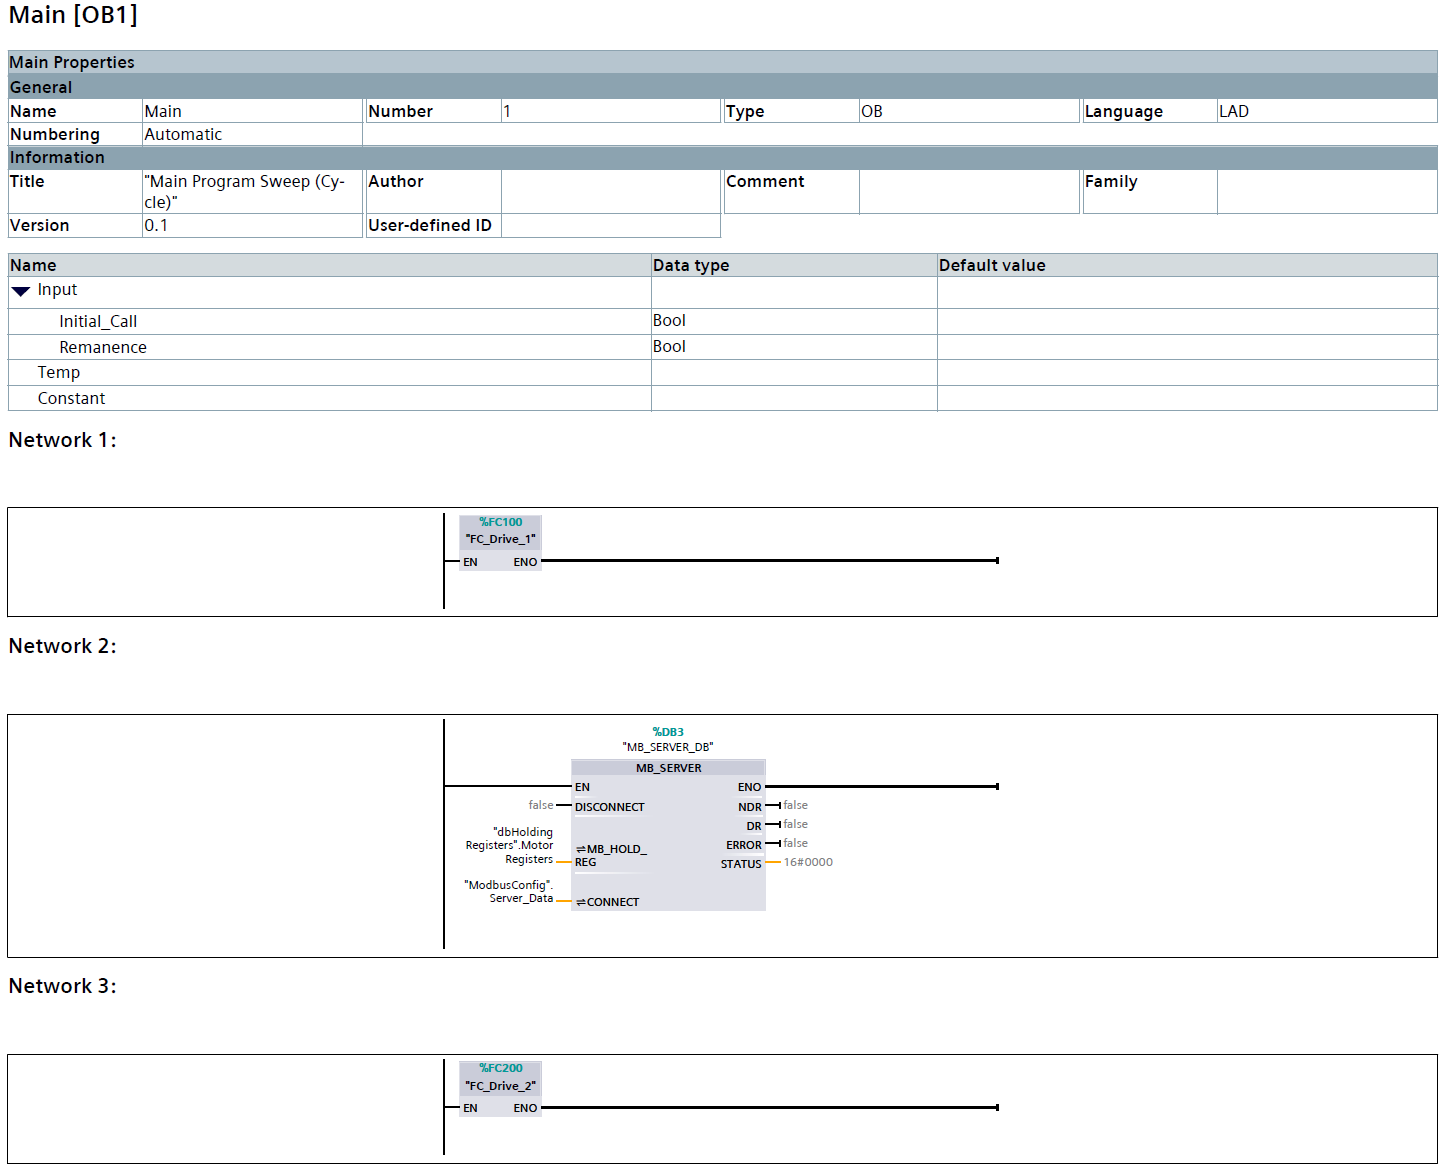
\includegraphics[width=0.5\linewidth]{FBDs/MainProgramSweep.PNG}
    \caption{Main Program Sweep cycle in the PLC}
    \label{fig:OB1}
\end{figure}


\newgeometry{scale=0.75}
\thispagestyle{empty}
{%
\begin{figure}[H]
    \centering
    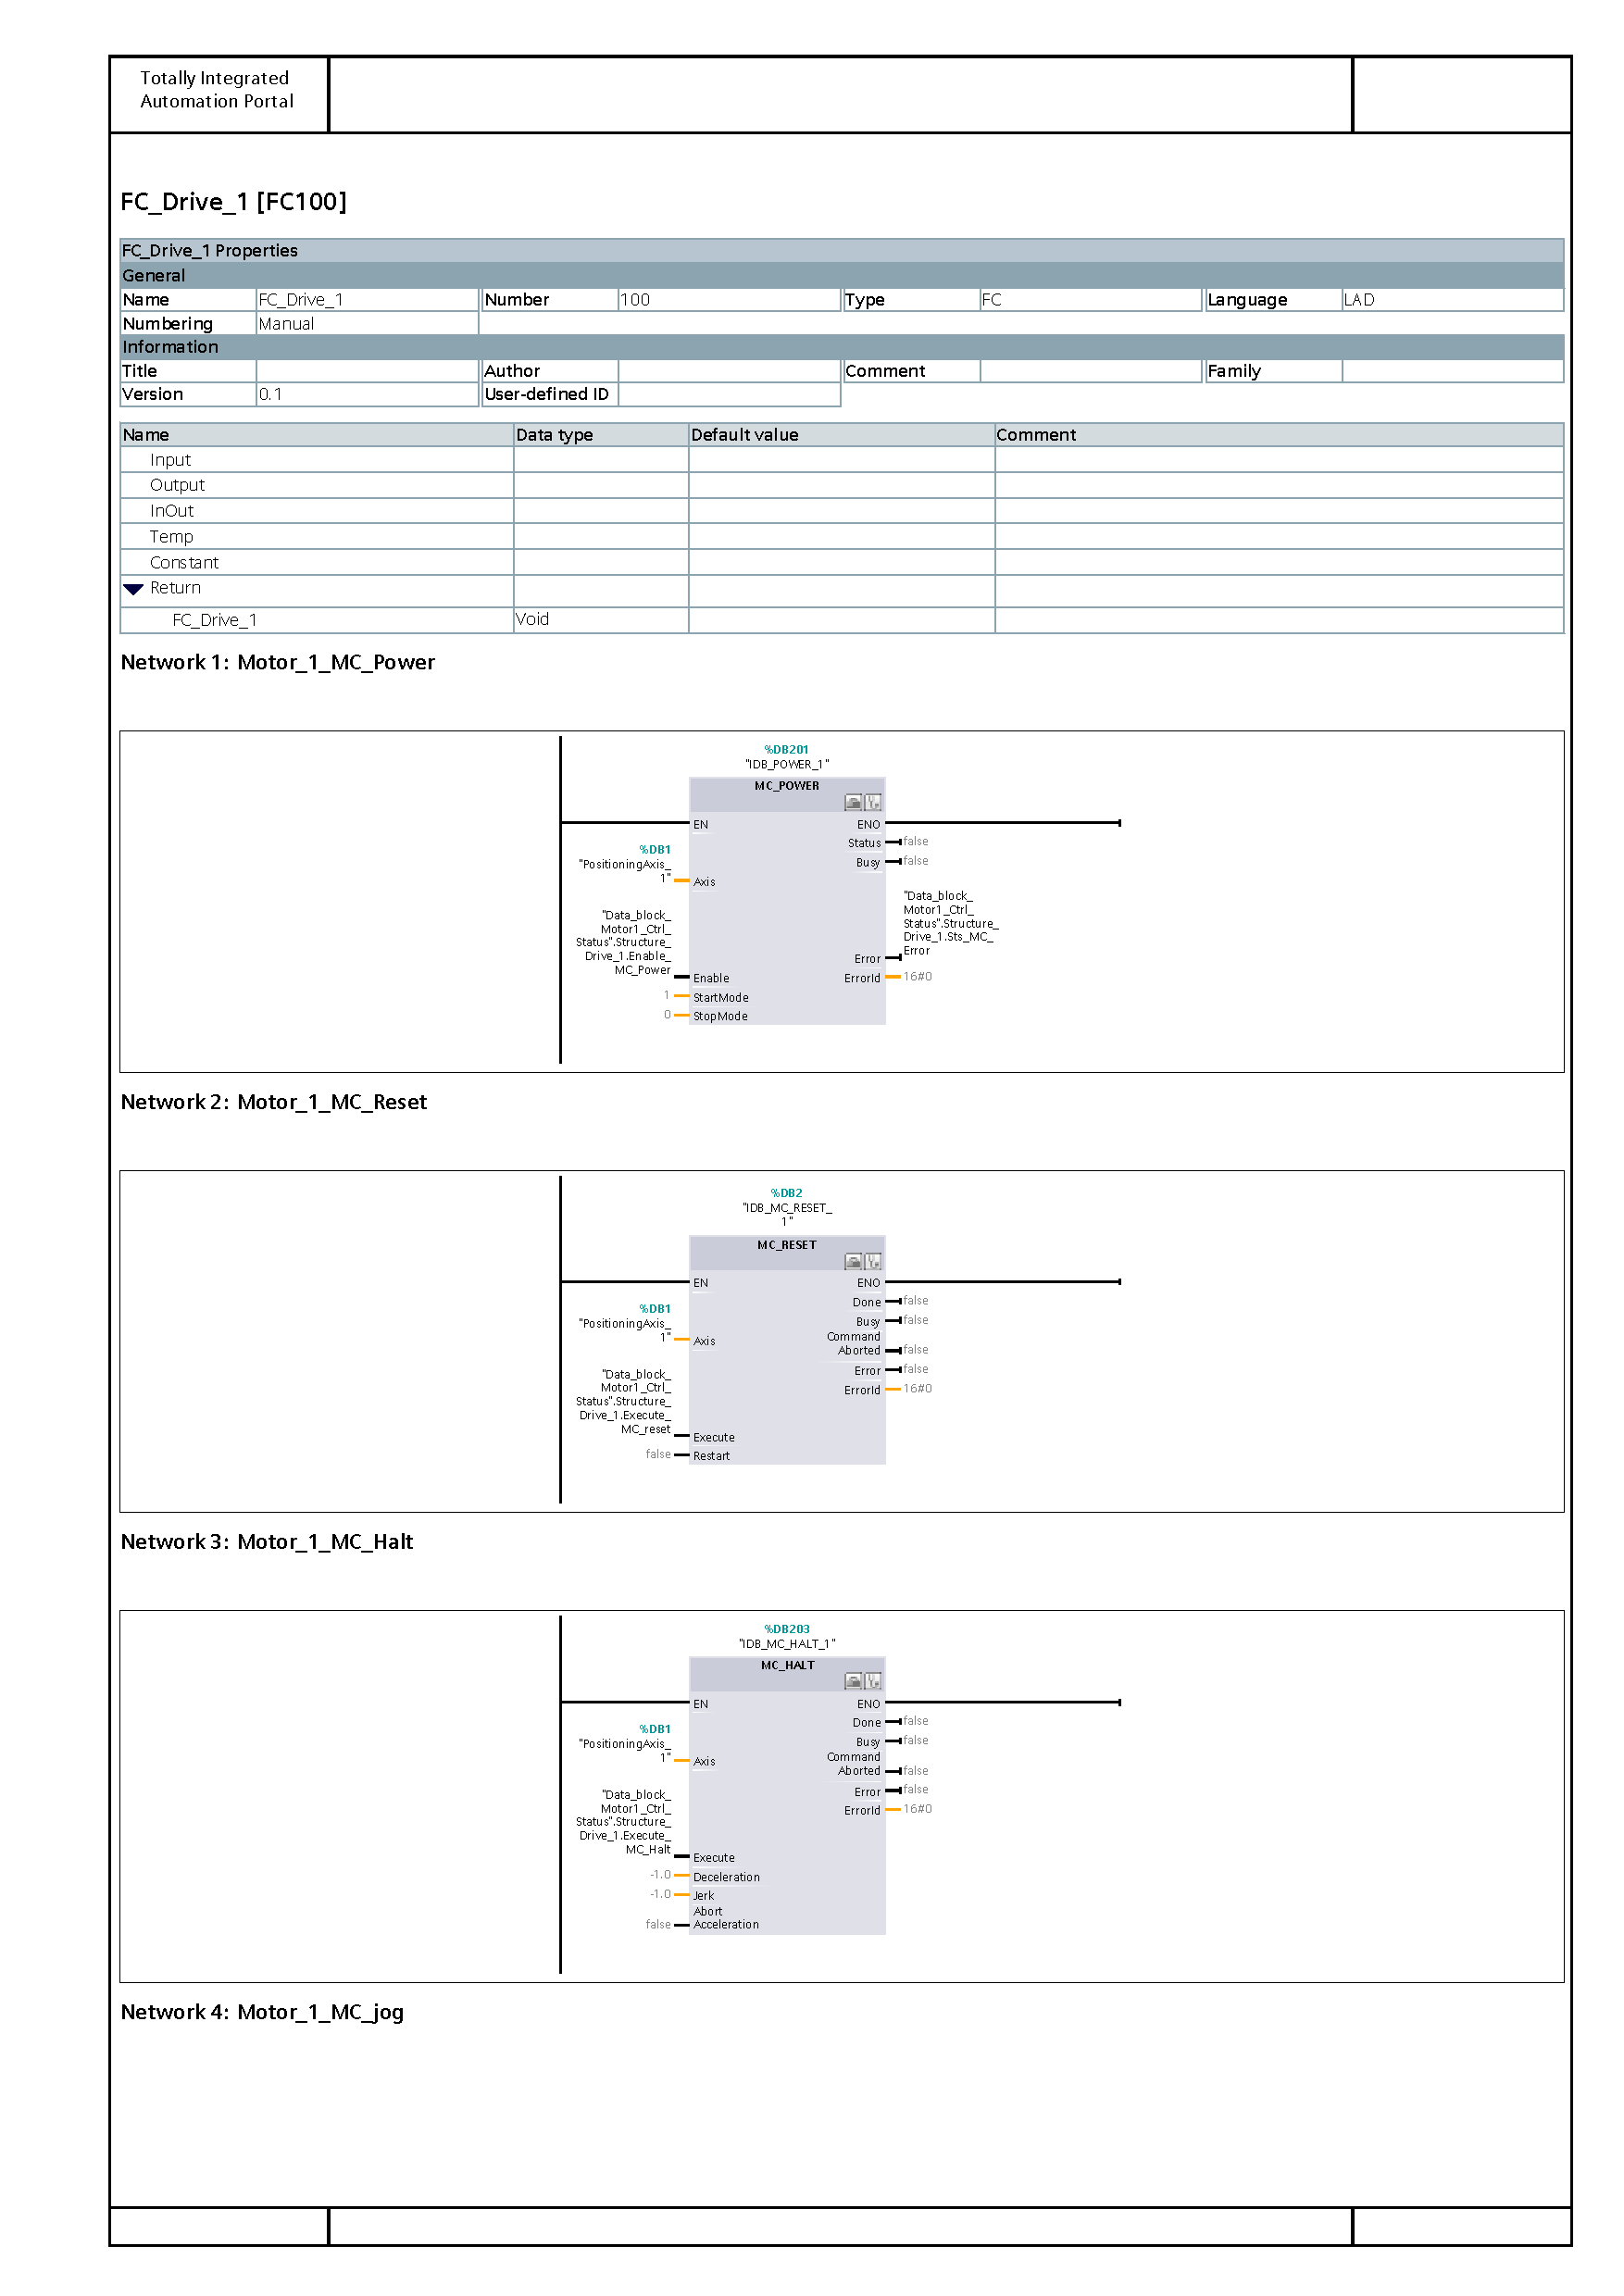
\includegraphics[page=1,scale=.5]{FBDs/FC_1.pdf}
    \caption{The function block for the control of Drive 1, the function block for Drive 2 is similar with appropriate change of variables.}
    \label{fig:FC1}
\end{figure}
  \par
}
\includepdf[pages={2-4},scale=.75]{FBDs/FC_1.pdf}
\restoregeometry

\begin{figure}[H]
    \centering
    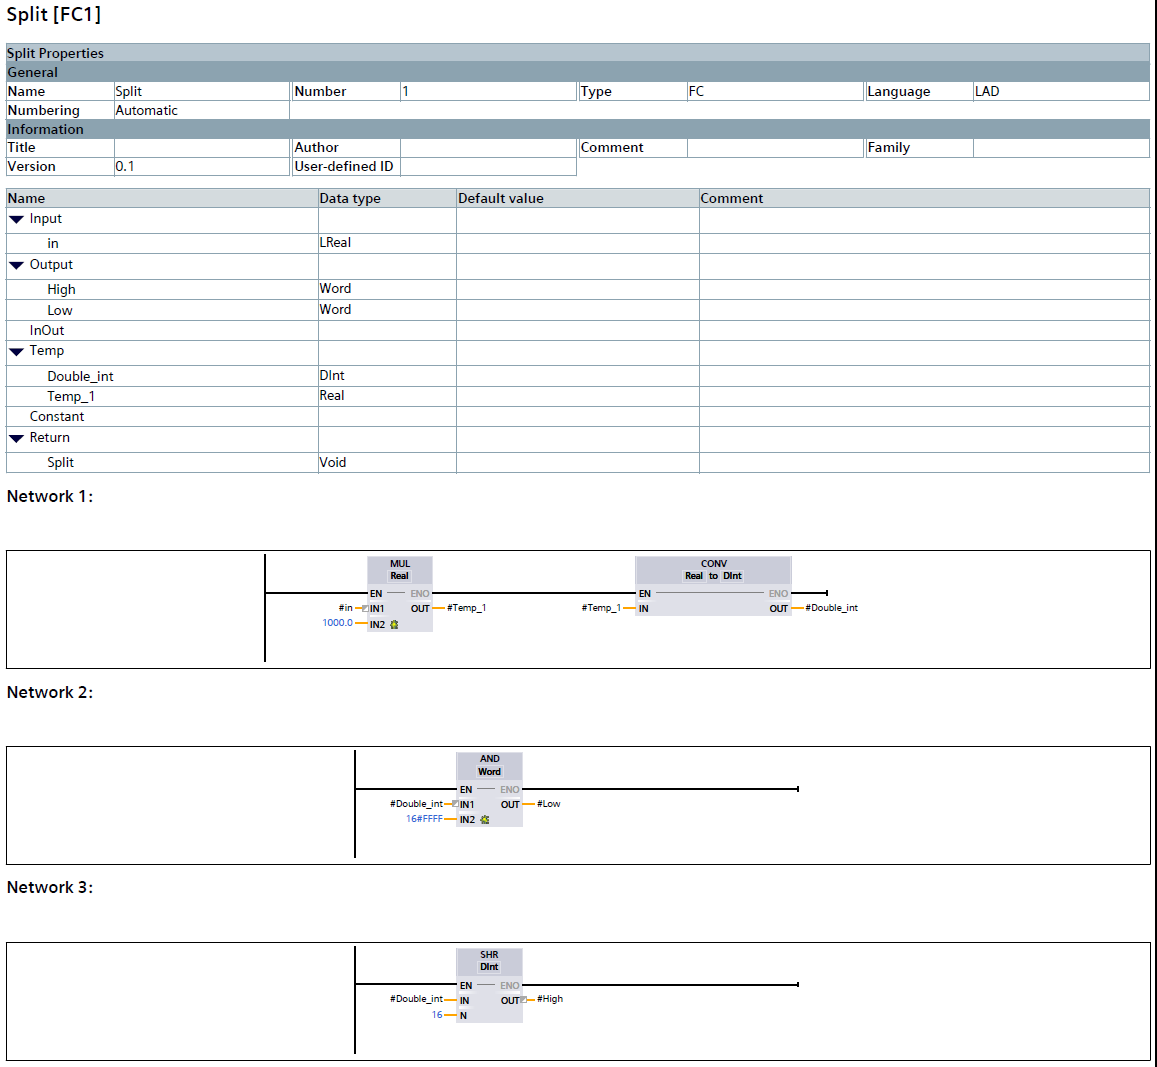
\includegraphics[width=0.5\linewidth]{FBDs/split.PNG}
    \caption{Function block for splitting a 32-bit \Gls{real} into two 16 bit \glspl{word}}
    \label{fig:split}
\end{figure}
\begin{figure}[H]
    \centering
    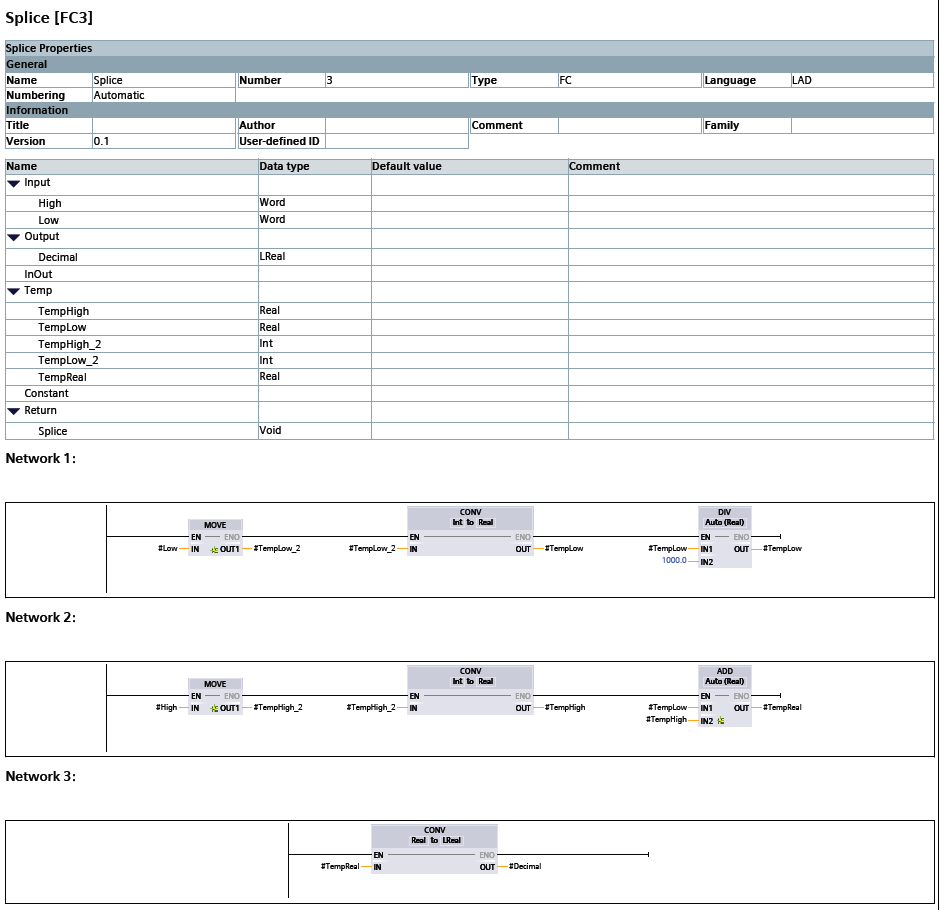
\includegraphics[width=0.5\linewidth]{FBDs/Splice.PNG}
    \caption{Function block for splicing together a 32-bit \Gls{real}(floating point value) from two 16 bit \glspl{word} before converting it to a 64 bit \Gls{lreal}.}
    \label{fig:Splice}
\end{figure}

\begin{figure}[H]
    \centering
    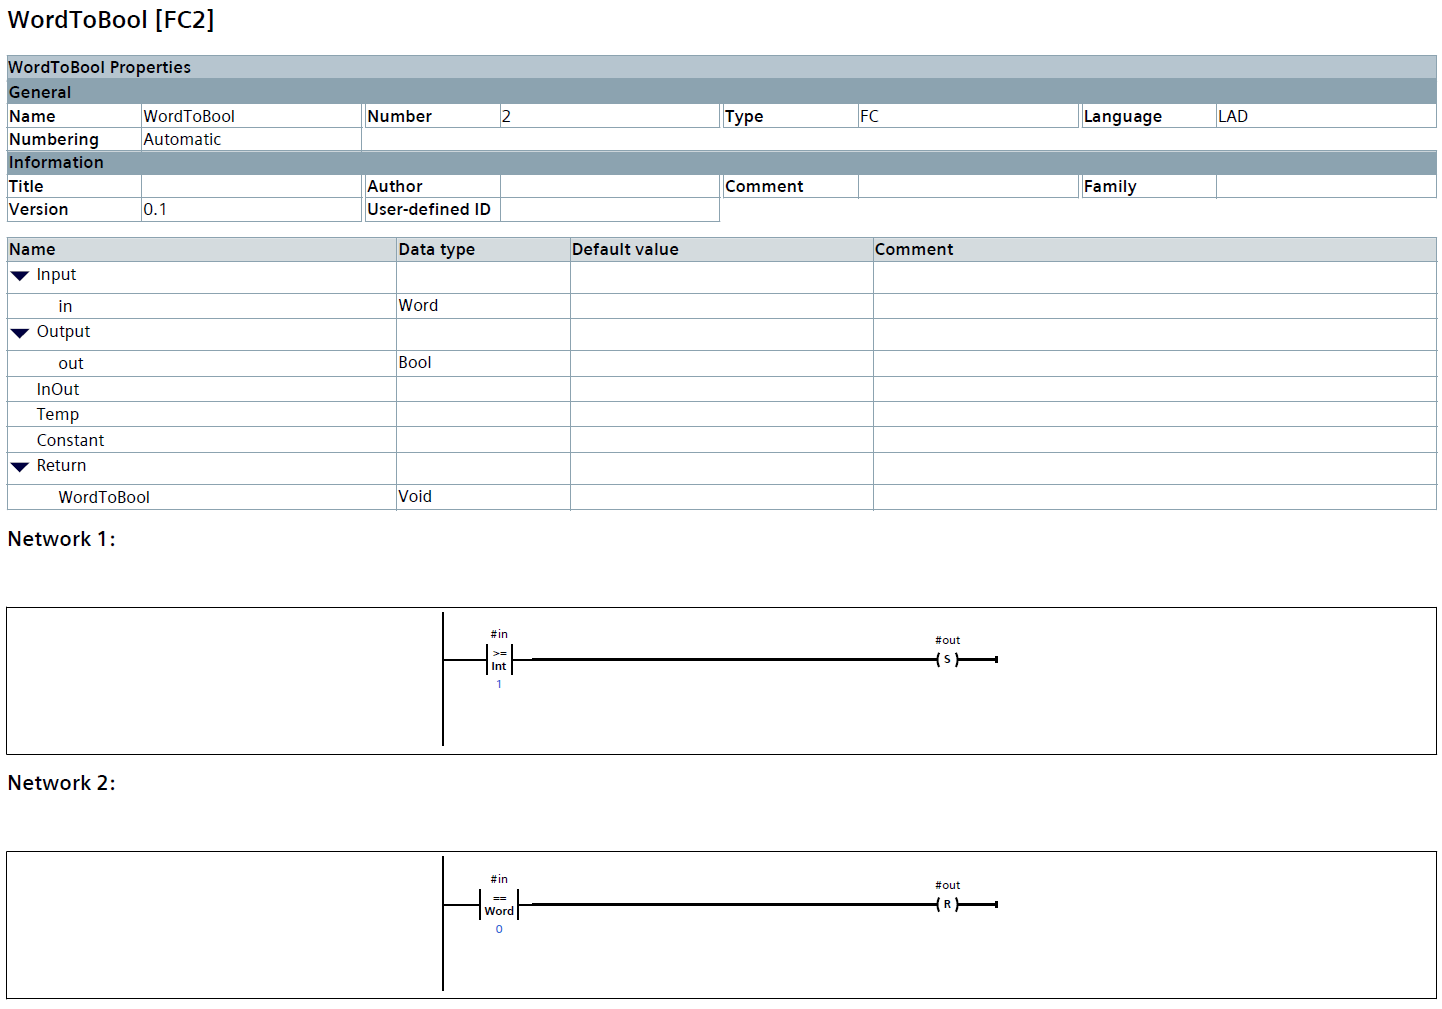
\includegraphics[width=0.5\linewidth]{FBDs/WordToBool.PNG}
    \caption{Function block for converting a 16-bit \gls{word}(which only takes the values 0 or 1) into a 1-bit \gls{bool}}
    \label{fig:WTB}
\end{figure}
\section{Data Blocks}
\begin{figure}[H]
    \centering
    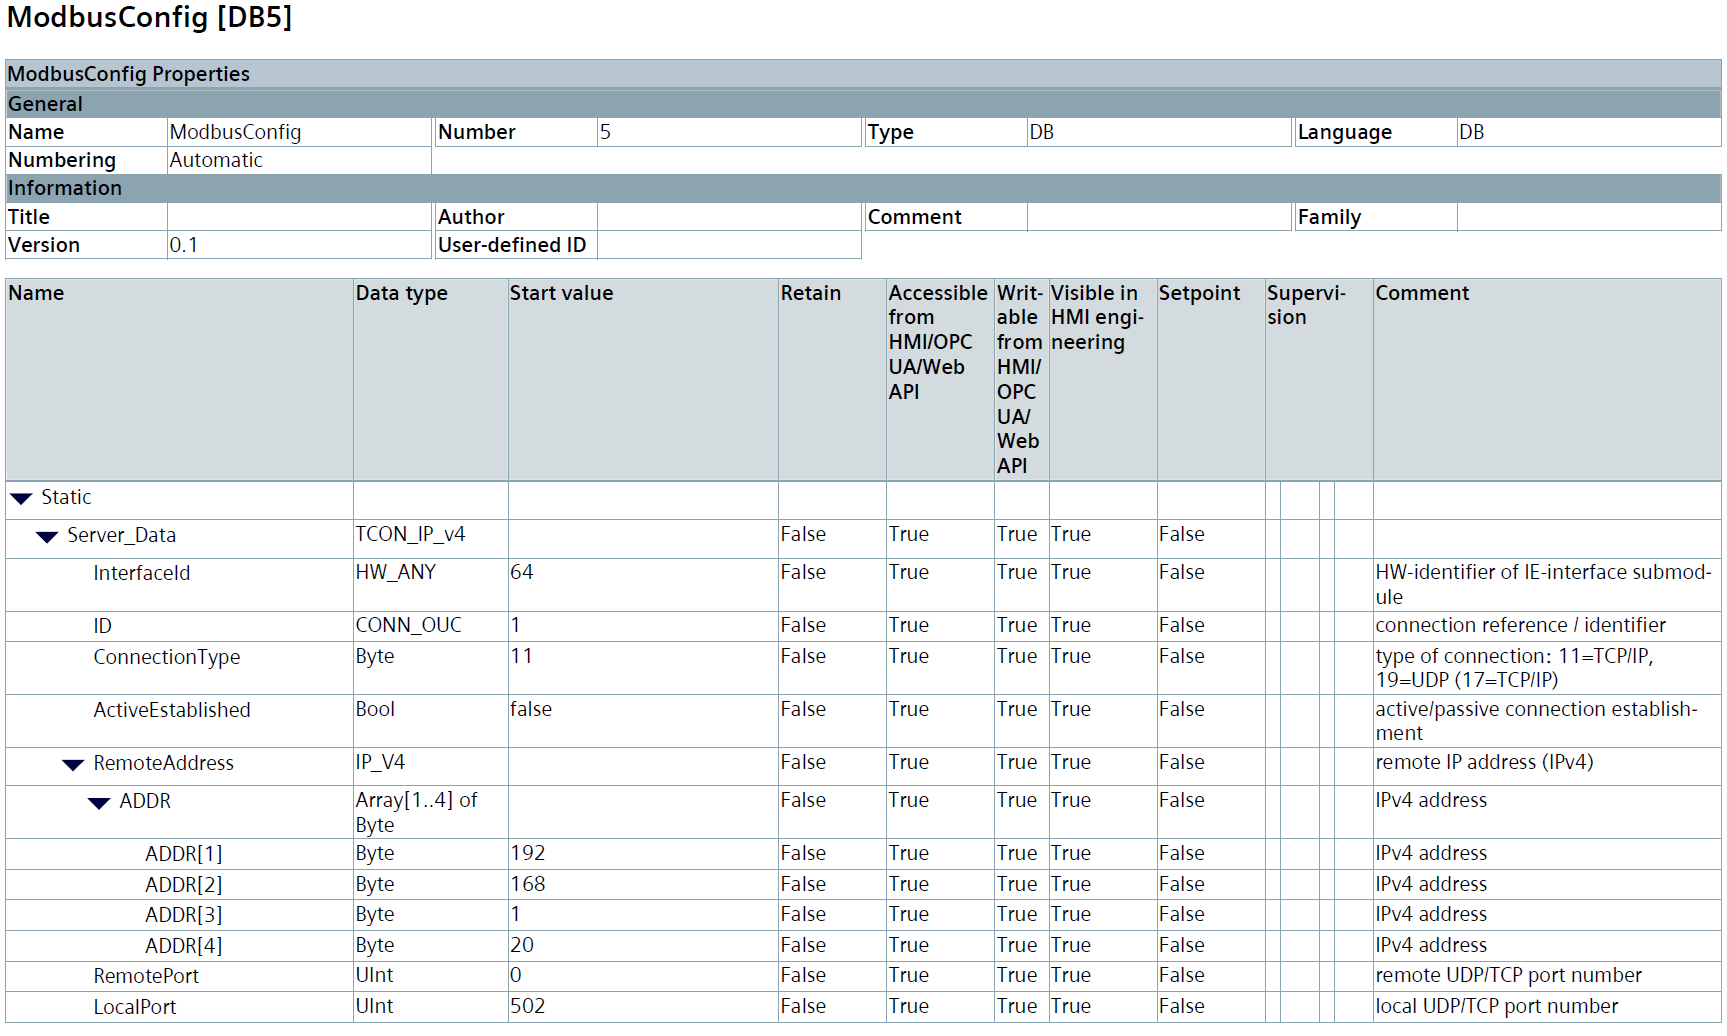
\includegraphics[width=0.5\linewidth]{DBs/ModbusConfig.PNG}
    \caption{Data block that sets up the Mobus Server on the PLC}
    \label{fig:ModbusConfig}
\end{figure}
\begin{figure}[H]
    \centering
    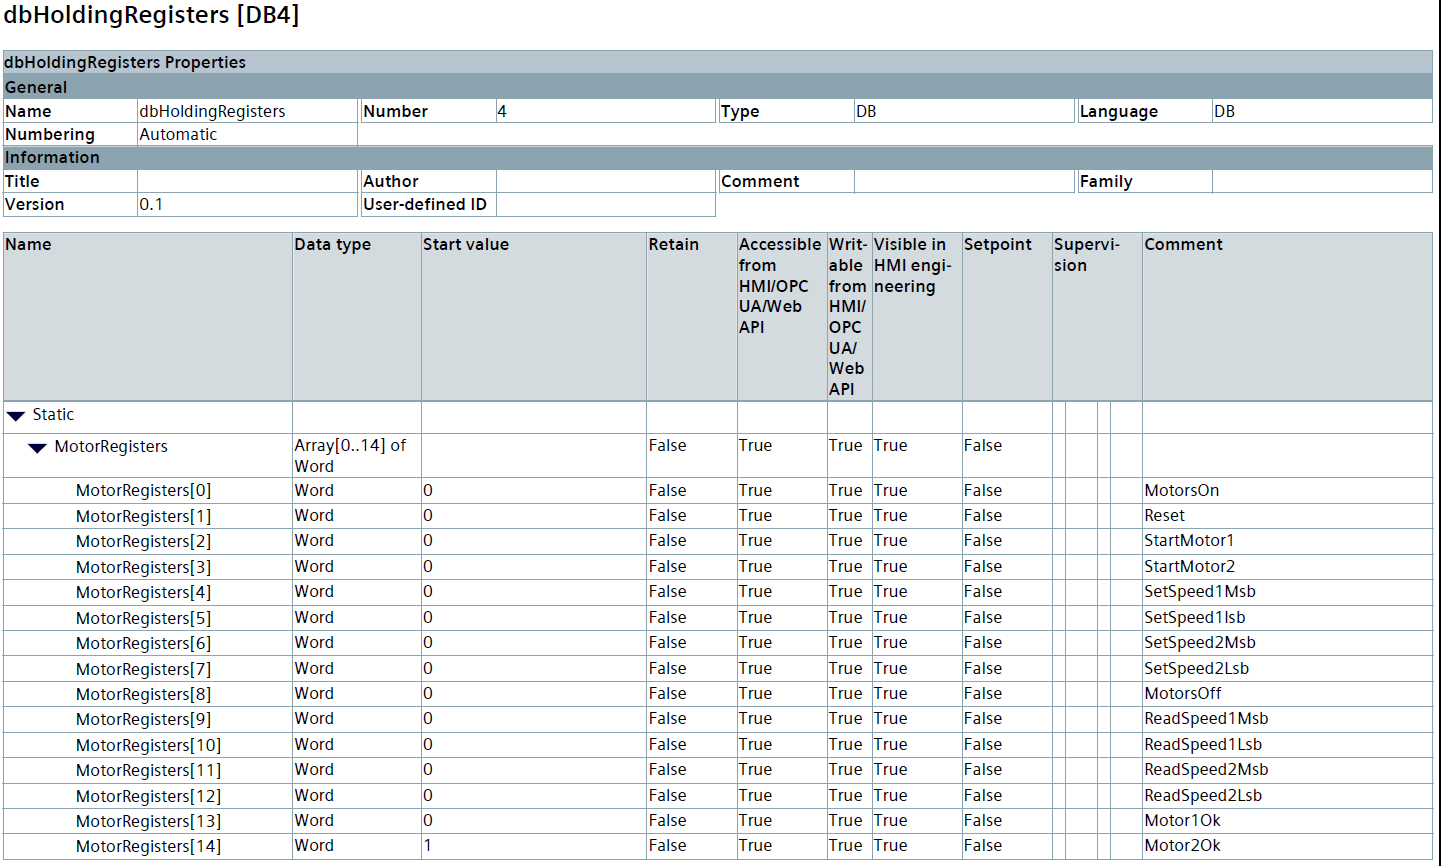
\includegraphics[width=0.5\linewidth]{DBs/dbHoldingRegisters.PNG}
    \caption{Data block for the different registers sent back and forth on the Modbus connection}
    \label{fig:dbHoldReg}
\end{figure}
\begin{figure}[H]
    \centering
    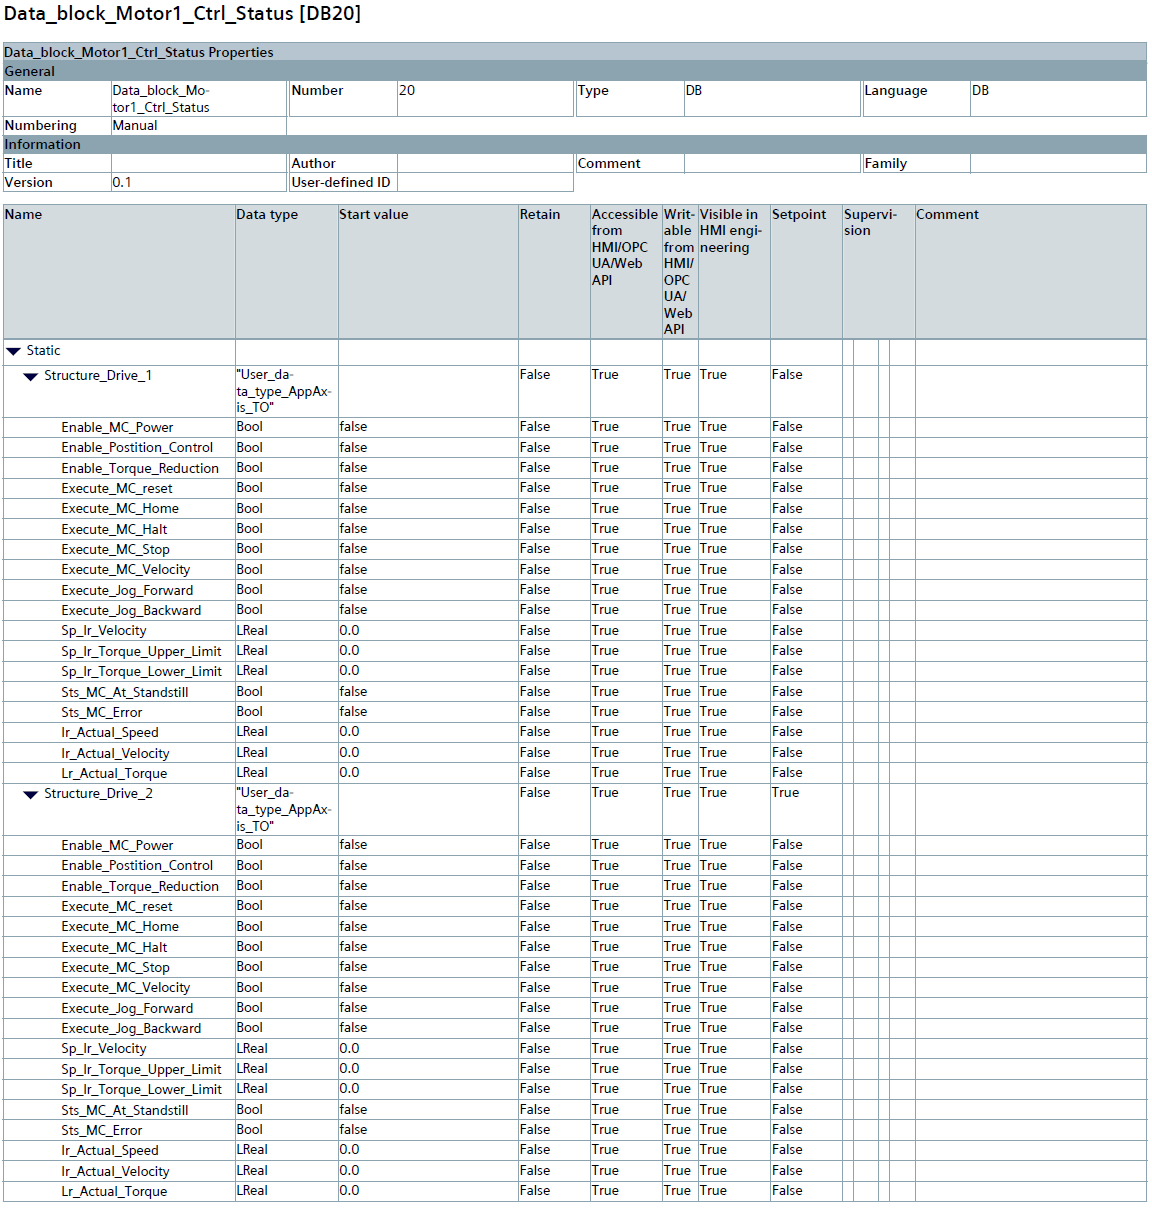
\includegraphics[width=0.5\linewidth]{DBs/MotorCtrlStatus.PNG}
    \caption{Data block for the status of both motor drives on the PLC}
    \label{fig:MotorSTS}
\end{figure}
\begin{figure}[H]
    \centering
    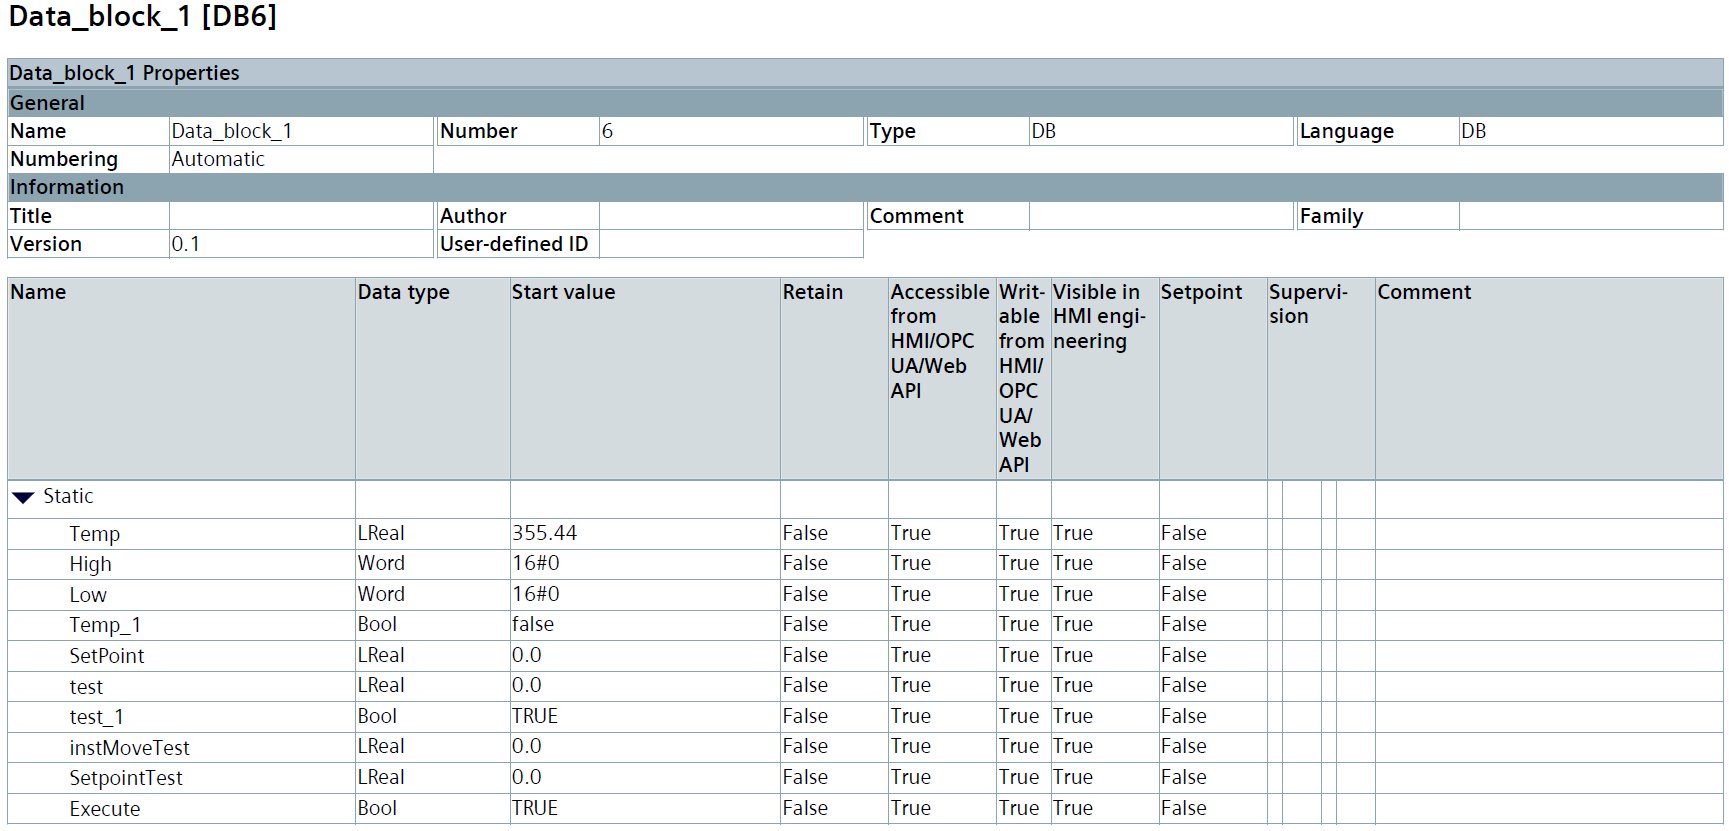
\includegraphics[width=0.5\linewidth]{DBs/temp.PNG}
    \caption{Data block for holding temporary values for PLC arithmetic and test values}
    \label{fig:temp}
\end{figure}
\section{Labview}

\subsection{Typedefs}
\begin{multicols}{2}
\begin{figure}[H]
    \centering
    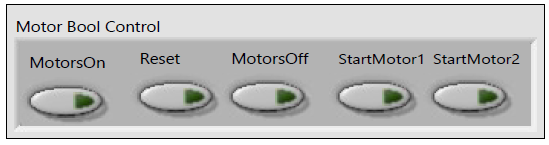
\includegraphics[width=0.5\linewidth]{vis/Motor Bool control.PNG}
    \caption{Typedef of the booleans sent over the Modbus connection.}
    \label{fig:MotorBoolCl}
\end{figure}
\begin{figure}[H]
    \centering
    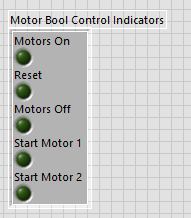
\includegraphics[width=0.5\linewidth]{vis/Motor Bool Indicatorsl.PNG}
    \caption{Typedef of the booleans received over the Modbus connection.}
    \label{fig:MotorBoolInd}
\end{figure}
\begin{figure}[H]
    \centering
    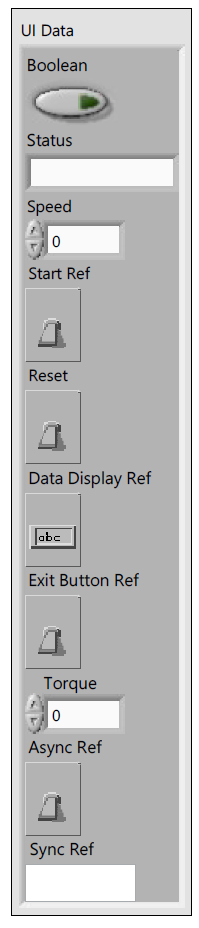
\includegraphics[scale=0.5]{vis/UI.PNG}
    \caption{Typedef of elements of the UI}
    \label{fig:UI}
\end{figure}
\end{multicols}
\subsection{Helper VIs}
\begin{figure}[H]
    \centering
    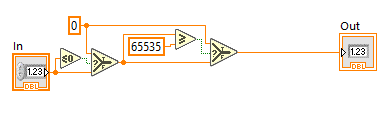
\includegraphics[width=0.5\linewidth]{vis/Remove invalid values.PNG}
    \caption{Helper VI that removes invalid values. Since an unsigned 16-bit word that is sent over the Modbus connection can hold an integer value up to $2^{16} = 65535$. Any value outside this range is forced to be either $0$ or $65535$.}
    \label{fig:RIV}
\end{figure}
\begin{figure}[H]
    \centering
    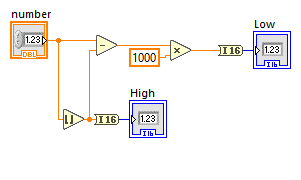
\includegraphics[width=0.5\linewidth]{vis/SplitDouble.PNG}
    \caption{Helper VI that splits a 64 bit-double into two 16-bit words \textbf{High} and \textbf{Low} for Modbus communication. The double is first rounded down to a integer to get the \textbf{High}-part and then that is subtracted from the original number the remaining \textbf{Low}-part is then multiplied by $1000$ because you can't send decimals on this form. On the receiving side the \textbf{Low}-part is divided by $1000$ again as shown in \figref{fig:Splice}.}
    \label{fig:SplitDouble}
\end{figure}

\begin{figure}[H]
    \centering
    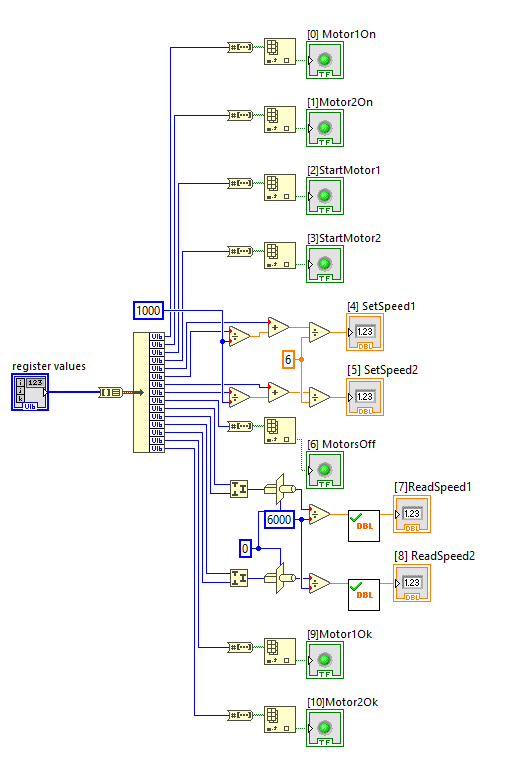
\includegraphics[width=0.5\linewidth]{vis/RegisterSplit.PNG}
    \caption{Helper VI that splits the register received over modbus to appropriate values for the Labview application.}
    \label{fig:RegisterSplit}
\end{figure}

\subsection{Important VIs}
\begin{figure}[H]
    \centering
    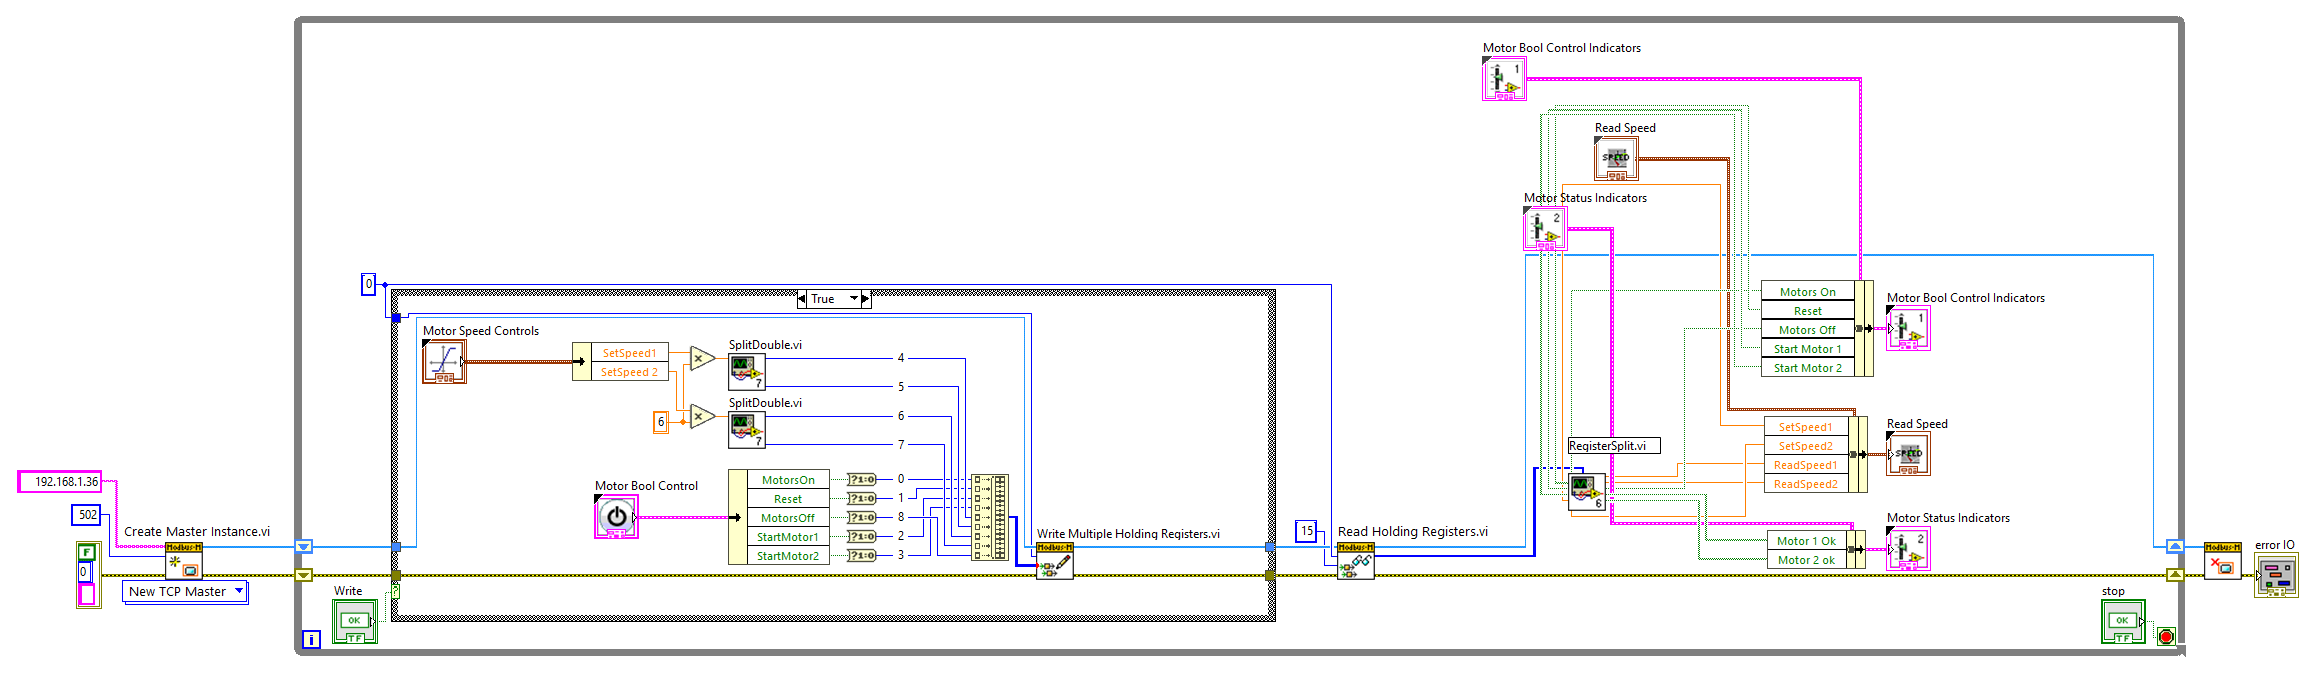
\includegraphics[width=0.75\linewidth]{vis/ModbusIO.PNG}
    \caption{How the modbus connection works on the labview side. This has been adapted to fit better into the \acrshort{mcl}, but functionality is the same.}
    \label{fig:ModbusIO}
\end{figure}

\begin{figure}[H]
    \centering
    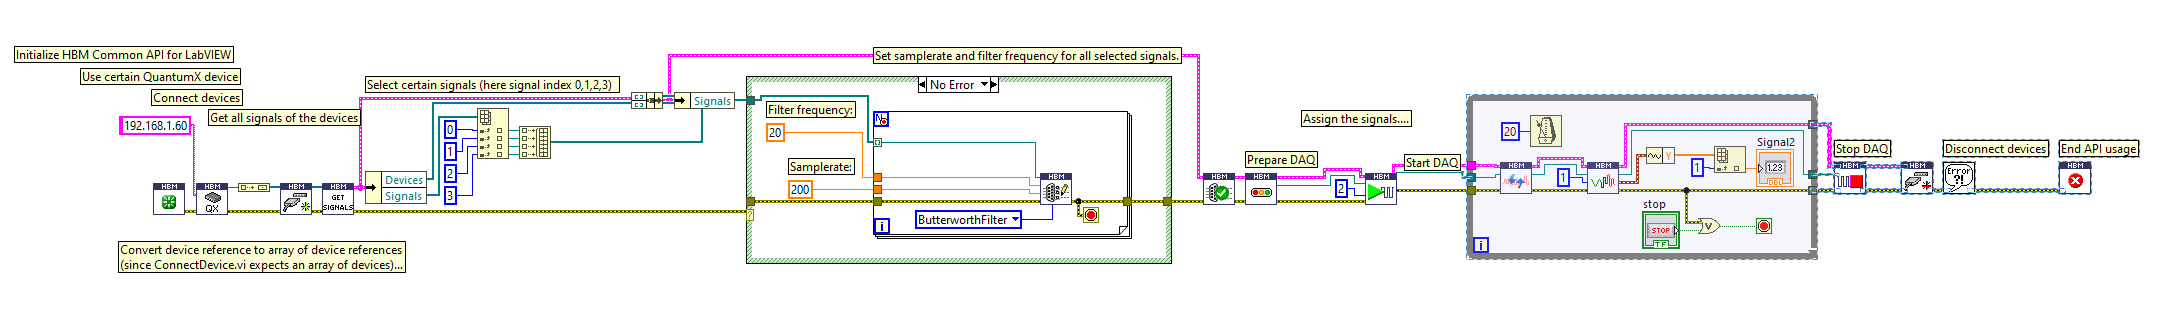
\includegraphics[width=0.75\linewidth]{vis/LoggingSystem.PNG}
    \caption{How the loggin system works. This has been adapted to fit better into the logging loop, but functionality is the same. This example also takes measurements from one channel, the full system utilises all four available channels.}
    \label{fig:Logging}
\end{figure}
\end{document}
